%% Be sure to check spelling!

%% Put **your** name and the proper due date in place

\documentclass{article}
\usepackage{amsmath}    % loads AMS-Math package
\usepackage{epsfig}     % allows PostScript files
\usepackage{listings}   % allows lstlisting environment
\usepackage{moreverb}   % allows listinginput environment
\usepackage[letterpaper, margin=0.75in]{geometry}  % set paper size/margins

\begin{document}
\begin{center}
\rule{6.5in}{0.5mm}\\~\\
\textbf{\large EGR 103L -- Fall 2017}\\~\\
\textbf{\huge \LaTeX~Assignment}\\~\\
Ian Hanus (ih52)\\
Lab Section 001, Tuesday 8:30-11:20 AM\\
September 10th, 2017\\~\\
{\small I understand and have adhered to all the tenets of the Duke
  Community Standard in completing every part of this assignment.  I
  understand that a violation of any part of the Standard on any part
  of this assignment can result in failure of this assignment, failure
  of this course, and/or suspension from Duke University.} 
\rule{6.5in}{0.5mm}\\
\end{center}
\tableofcontents
\listoffigures
\pagebreak

\section{Equations} %%% You will add your equations here
\begin{itemize}
\item General second-order system equation\cite[p.~221]{Rizzoni}:
% unnumbered and aligned equation
\begin{align*}
\frac{1}{\omega^2_n}\frac{d^2x(t)}{dt^2}+\frac{2\zeta}{\omega_n}\frac{dx(t)}{dt}+x(t)=K_{\mbox{s}}f(t)
\end{align*}
\item The Secant Formula for finding maximum stress 
in a column\cite[p.~681]{Hibbeler}:
% unnumbered and aligned equation
\begin{align*}
\sigma_{\mbox{\small{max}}}=\frac{P}{A}\Bigg[1+\frac{ec}{r^2}\mbox{sec}\Bigg(\frac{L}{2r}\sqrt{\frac{P}{EA}}\Bigg)\Bigg]
\end{align*}
\item Characteristic determinant for a 2x2 system of 
differential equations\cite[p.~152]{Kreyszig}:
\begin{align}
\mbox{det}(\boldsymbol{A}-\lambda\boldsymbol{I})&=
\begin{vmatrix}a_{11}-\lambda&a_{12}\\\nonumber
a_{21}&a_{22}-\lambda\end{vmatrix}\\\nonumber
&= (a_{11}-\lambda)(a_{22}-\lambda)-a_{12}a_{21}\\
&= \lambda^2-(a_{11}+a_{22})\lambda+a_{11}a_{22}-a_{12}a_{21}=0
\end{align}
% aligned numbered equations...except no numbers on first par
\item Definition of the Lyapunov exponent\cite[p.~56]{Ott}:
\begin{align}
h &= \lim_{T \to \infty}\frac{1}{T}\ln \bigg|\frac{\mbox{d}x_T}{\mbox{d}x_0}\bigg|\\
h &= \lim_{T \to \infty}\frac{1}{T}\sum_{n=0}^{T-1}\ln |M'(x_n)|\\
h &= \int \ln |M'(x)|d\mu(x)
\end{align}
% aligned numbered equations
\end{itemize}
\section{Tables using \texttt{tabular} and \texttt{array}}
\subsection{Using \texttt{tabular}} %%% You will add the tabular here
Converting ammonia into nitric acid - the Ostwald Process\cite{Ostwald}:
% centered tabular here
\begin{center}
\begin{tabular}{r|l}
Description & Chemical equation\\ \hline
Oxidization of Ammonia & $\mbox{4 NH}_3  \mbox{ (g)} + 5  \mbox{ O}_2  \mbox{(g)} \rightarrow 4  \mbox{ NO (g)} + 6  \mbox{ H}_2\mbox{O (g)}$\\
Oxidization of Nitric Oxide & $2 \mbox{ NO} \mbox{ (g)} + \mbox{ O}_2 \mbox{ (g)} \rightarrow 2 \mbox{ NO}_2 \mbox{ (g)}$\\
Absorption of Nitrogen Dioxide & $3 \mbox{ NO}_2 \mbox{ (g)} + \mbox{H}_2 \mbox{O (l)} \rightarrow 2 \mbox{ HNO}_3 \mbox{ (aq)} + \mbox{NO (g)}$
\end{tabular} 
\end{center}
\subsection{Using \texttt{array}} %%% You will add the array here
% stretched array here
\begin{center}
\[
\renewcommand{\arraystretch}{1.5}
\begin{array}{|c|c|}\hline
\mbox{Equation} & \mbox{Description}\\ \hline \hline
\vec{v}=v_x\hat{\imath}+v_y\hat{\jmath}+v_z\hat{k} & \mbox{Resolution into Components}\\ \hline
v^2=v_0^2+2a\Delta x & \mbox{Velocity formula}\\ \hline
\end{array}
\]
\end{center}
\pagebreak

\section{Comments} %%% You will add your comments here
Things I learned in this assignment:
% itemized list here
\begin{itemize}
\item How to use the \texttt{align} and \texttt{align*} environment to typeset numbered and unnumbered equations and using the \texttt{nonumber} command to suppress numbering equations in an  \texttt{align} environment;
\item How to use \$ to enter math mode in a line of text to type shorter mathematical expressions like $10^6$ and $\nabla u$ or Greek letters like $\Delta$;
\item How to use the \texttt{mathrm} command to put super- and subscripts in regular, versus italic, type for things like $V_{\mathrm{min}}$ instead of $V_{min}$;
\item How to change the appearance of fonts to make words \textbf{bold}, \textit{italics}, \underline{underlined}, or \texttt{typewriter font};
\item How to use the \texttt{tabular} environment to create tables of varying sizes and formats;
\item How to use the \texttt{array} environment to create arrays; and
\item How to adjust font size with commands such as \texttt{Bigg} and \texttt{small}.
\end{itemize}
\pagebreak
\appendix
\section{Codes}
%%% Everything in this section is done; make sure you 
%%% understand how it works in general
\subsection{Listing of full sample header for original code}
\listinginput[1]{1}{Header1f.m}

\subsection{Listing of short sample header for original code}
\listinginput[1]{1}{Header1s.m}

\subsection{Listing of full sample header for modified code}
\listinginput[1]{1}{Header2f.m}

\subsection{Listing of short sample header for modified code}
\listinginput[1]{1}{Header2s.m}

\pagebreak
\section{Figures \label{FigureList}}
%%% Almost everything in this section is done; make sure you 
%%% understand how it works in general and be sure to 
%%%uncomment the epsfig lines

\begin{figure}[htb]
\begin{center}
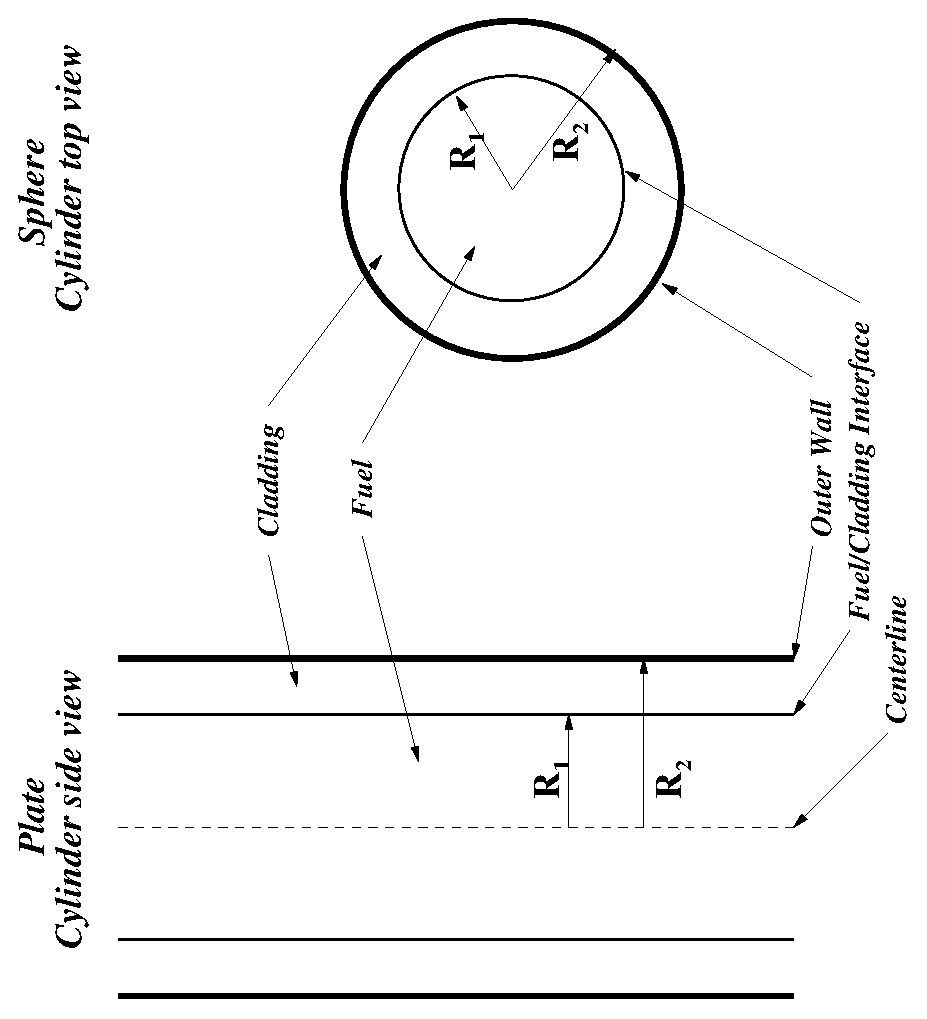
\epsfig{file=drawing.eps, width=3in, angle=-90} 
\caption{Drawing from ME 431L test.}
\end{center}
\end{figure}

\begin{figure}[htb]
\begin{center}
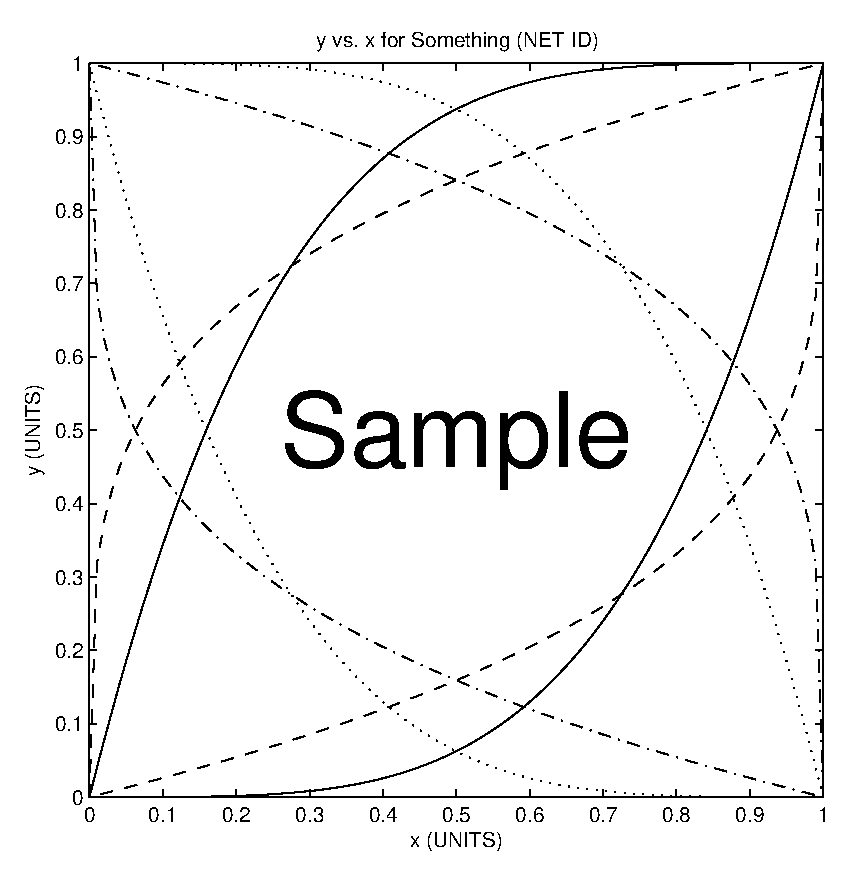
\epsfig{file=SampleFigure.eps, width=2.5in} 
\caption{Sample MATLAB figure.}
\end{center}
\end{figure}
\pagebreak

%%% Everything in this section is done; make sure you 
%%% understand how it works in general
%%% Note that line returns are optional
\addcontentsline{toc}{section}{References}
\begin{thebibliography}{9}
\bibitem{Rizzoni}
Rizzoni, Georgio,
{\it Principles and Applications of Electrical Engineering}.
McGraw-Hill, New York,
5th Edition,
2007.
\bibitem{Hibbeler}
Hibbeler, R. C.,
{\it Mechanics of Materials}.
Pearson Prentice Hall, Upper Saddle River, NJ, 8th Edition, 2011.
\bibitem{Kreyszig}
Kreyszig, Erwin,
{\it Advanced Engineering Mathematics}.
John Wiley \& Sons, New York, 8th Edition, 1999.
\bibitem{Ott}
Ott, Edward,
{\it Chaos in Dynamical Systems}.
Cambridge University Press, Cambridge, UK, 1st Edition, 1993.
\bibitem{Ostwald}
Wikipedia, 
{\it Ostwald process} (http://en.wikipedia.org/wiki/Ostwald$\_$process).
Online; accessed 19-Aug-2012.
\end{thebibliography}

\end{document}
